\documentclass[11pt,a4paper]{article}

% ── Packages ─────────────────────────────────────────────────────────
\usepackage[utf8]{inputenc}
\usepackage[T1]{fontenc}
\usepackage{amsmath,amssymb,amsthm}
\usepackage{mathtools}
\usepackage{booktabs}
\usepackage{hyperref}
\usepackage{cleveref}
\usepackage{enumitem}
\usepackage[margin=1in]{geometry}
\usepackage{xcolor}
\usepackage{graphicx}
\usepackage{listings}

% ── Theorem environments ─────────────────────────────────────────────
\newtheorem{theorem}{Theorem}[section]
\newtheorem{lemma}[theorem]{Lemma}
\newtheorem{proposition}[theorem]{Proposition}
\newtheorem{corollary}[theorem]{Corollary}
\theoremstyle{definition}
\newtheorem{definition}[theorem]{Definition}
\newtheorem{remark}[theorem]{Remark}
\newtheorem{hypothesis}{Hypothesis}

% ── Lean code listings ───────────────────────────────────────────────
\lstdefinelanguage{lean4}{
  keywords={theorem,def,lemma,axiom,import,namespace,end,by,sorry,
            intro,exact,refine,calc,have,obtain,use,unfold,rfl,
            noncomputable,where,if,then,else,let,in},
  morecomment=[l]{--},
  morecomment=[s]{/-}{-/},
  morestring=[b]",
  sensitive=true,
}
\lstset{
  language=lean4,
  basicstyle=\ttfamily\small,
  keywordstyle=\bfseries\color{blue!70!black},
  commentstyle=\itshape\color{gray},
  breaklines=true,
  frame=single,
  numbers=left,
  numberstyle=\tiny\color{gray},
  xleftmargin=2em,
}

% ── Macros ───────────────────────────────────────────────────────────
\newcommand{\R}{\mathbb{R}}
\newcommand{\Q}{\mathbb{Q}}
\newcommand{\N}{\mathbb{N}}
\newcommand{\NS}{Navier--Stokes}
\newcommand{\Lip}{\mathrm{Lip}}
\newcommand{\grad}{\nabla}
\newcommand{\lapl}{\nabla^2}
\newcommand{\norm}[1]{\lVert #1 \rVert}
\newcommand{\abs}[1]{\lvert #1 \rvert}
\newcommand{\Rey}{\mathrm{Re}}
\DeclareMathOperator{\diver}{div}

% ── Review-pass markup (render but remain visible in source) ─────────
\newcommand{\strongclaim}[1]{\textbf{#1}}  % Will survive adversarial review
\newcommand{\weakclaim}[1]{\emph{#1}}      % Reviewer will probe; see source note
\newcommand{\openquestion}[1]{%
  \textcolor{black!70}{[\textsc{open}: #1]}}

% ═════════════════════════════════════════════════════════════════════
\title{A Scaling Invariant at Direction-Field Creases in 3D \NS{}
  Reconnection:\\ Conditional Regularity Failure, Emergent Balance,
  and Lean~4 Formalisation}

\author{Adam Roediger\thanks{Live Oak Legacy Builders LLC.}
  \and Patrick Moriarty\thanks{Bitumen Machina LLC, Coastal Georgia.}}

\date{April 2026}

\begin{document}
\maketitle

% ── Abstract ─────────────────────────────────────────────────────────
\begin{abstract}
We study the structure of the viscous term $\nu\lapl\omega$ at
direction-field creases in 3D incompressible \NS{} vortex
reconnection.  Decomposing vorticity as $\omega=\abs{\omega}\,\xi$,
the product rule produces $\abs{\omega}\lapl\xi$---a term whose
regularity depends on the direction field $\xi=\omega/\abs{\omega}$.
At the reconciliation surface between antiparallel vortex tubes, $\xi$
develops a crease: a thin layer where the direction field rotates
through $180^\circ$ between coherent tubes.

\strongclaim{Pseudospectral DNS at $\Rey=6400$ ($N=64,128,256$) shows
that the Lipschitz constant $\Lambda=\sup\abs{\grad\xi}_F$ scales as
$N^{0.86\pm0.05}$ ($R^2>0.96$), consistent with $O(1/\Delta x)$.}
However, this growth occurs where $\abs{\omega}\to0$---the
reconciliation gap between tubes.
\strongclaim{The product $\sup(\abs{\omega}\cdot\abs{\grad\xi}_F)$
is resolution-independent: $\gamma=0.04\approx0$ across a $4\times$
resolution range (coefficient of variation ${<}\,3\%$ at $t=0,10$).}
The individual factors scale as $N^{+\beta}$ and $N^{-\beta}$ at the
location of the product maximum, an interface ring between the tube
cores and the crease centre.

We formalise a conditional implication in Lean~4 with Mathlib: if
$\Lambda$ diverges \emph{and} $\abs{\omega}>0$ at the crease, then
$\nu\lapl\omega$ exits $L^2$.  The formal proof (13~theorems,
0~\texttt{sorry}, 10~Z3-certified bounds) is mathematically valid.
\weakclaim{The numerical data shows that the two antecedents are
coupled through the product invariant rather than independently
realised---whether they can be jointly instantiated is an open
question requiring late-reconnection field data at higher
resolution.}%
% NOTE: This is the weakest sentence in the abstract. The "coupled"
% language is accurate but a reviewer may ask: coupled how? The
% product invariant does not by itself establish a mechanism that
% prevents joint instantiation --- it shows that the current data
% does not exhibit it, which is weaker. Strengthening requires
% either (a) a proof that the invariant is a barrier, or (b)
% late-time field data where the invariant breaks.

The formal verification comprises 13~obligations,
10~Z3-certified numerical bounds, and 21~definitions grounded in
experimental data via exact rational arithmetic.  All source code,
certificates, and DNS data are included as ancillary files.
\end{abstract}

\smallskip\noindent
\textbf{MSC 2020:} 35Q30, 68V15, 76D05 \hfill
\textbf{Keywords:} \NS{}, regularity, vorticity direction field,
scaling invariant, vortex reconnection, formal verification, Lean~4

% ═════════════════════════════════════════════════════════════════════
\section{Introduction}\label{sec:intro}

The question of whether smooth solutions to the 3D incompressible
\NS{} equations remain smooth for all time, or whether finite-time
singularities can form, remains one of the central open problems in
mathematical fluid dynamics~\cite{DG1995, MB2002}.

Classical blowup criteria characterise singularity formation through
scalar norms: the Beale--Kato--Majda criterion~\cite{BKM1984}
requires $\int_0^T\norm{\omega}_{L^\infty}\,dt = \infty$, while
Constantin and Fefferman~\cite{CF1993} showed that regularity is
controlled by the vorticity direction field
$\xi = \omega/\abs{\omega}$---specifically, Lipschitz continuity
of~$\xi$ in regions of high vorticity suffices to prevent blowup.
The Constantin--Fefferman--Majda geometric criterion~\cite{CFM1996}
refined this to a local condition on the alignment of vorticity
with the strain eigenvectors.

Recent progress on the closely related Euler equations has
dramatically sharpened the picture.  Building on Hou and Luo's
numerical discovery of a potential singularity~\cite{HouLuo2014},
Chen and Hou~\cite{ChenHou2023} established finite-time blowup for
the 2D Boussinesq and 3D axisymmetric Euler equations via a nearly
self-similar mechanism.  Chen and Hou~\cite{ChenHou2025} subsequently
gave a rigorous computer-assisted proof of finite-time singularity
for 3D Euler with smooth initial data and boundary.
Elgindi~\cite{Elgindi2021} independently established finite-time
blowup for $C^{1,\alpha}$ Euler data (a lower regularity class).
For \NS{}, Tao~\cite{Tao2016} constructed finite-time blowup
solutions for an averaged version of the equations, demonstrating
that the known conservation laws do not by themselves prevent
singularity.  Hou~\cite{Hou2025} investigated nearly self-similar
blowup candidates for generalised axisymmetric \NS{}, and
Chen, Hou, and Huang~\cite{CHH2025} recently gave a
computer-assisted proof of nonuniqueness of Leray--Hopf solutions
to the unforced 3D \NS{} equations.

Our contribution starts from the Constantin--Fefferman direction-field
framework but shifts the focus from regularity criteria to direct
measurement of the direction field's structure under grid refinement.
The product rule decomposition $\omega=\abs{\omega}\xi$ exposes how
$\xi$'s regularity enters the viscous term: $\nu\lapl\omega$ contains
$\abs{\omega}\lapl\xi$, which becomes distributional if $\xi$ loses
smoothness while $\abs{\omega}$ remains positive.  We formalise this
conditional implication and then ask: what does the direction field
actually do at the crease?

\strongclaim{The answer is an emergent scaling balance.}  At the
reconciliation surface between antiparallel vortex tubes, $\xi$ must
rotate through $180^\circ$ over a thin layer.  The Lipschitz constant
$\Lambda=\sup\abs{\grad\xi}_F$ scales as $O(1/\Delta x)$---the
crease sharpens with resolution.  But the vorticity magnitude at the
crease location simultaneously decays, so that the product
$\sup(\abs{\omega}\cdot\abs{\grad\xi}_F)$ remains
resolution-independent.  This is distinct from, but complementary to,
the nonlinear blowup scenarios studied by Chen--Hou and Elgindi:
those works identify how the nonlinear term drives singularity; we
characterise the scaling structure of the viscous term at the crease.

\paragraph{What we prove.}
\strongclaim{Under three hypotheses---that $\Lambda$ diverges, that
$\abs{\omega}>0$ at the crease, and that a Gagliardo--Nirenberg
type estimate relates $\norm{\lapl\xi}_{L^2}$ to $\Lambda$---the
viscous term is unbounded in $L^2$, and the solution exits $H^2$
regularity.}  The formal proof in Lean~4 covers the algebraic core
(13~theorems, 0~\texttt{sorry}).  This conditional theorem is
mathematically valid regardless of the numerical evidence.

\paragraph{What we observe.}
Pseudospectral DNS of antiparallel vortex tube reconnection at
$\Rey=6400$ ($N=64,128,256$) on $[0,2\pi]^3$ shows:
\begin{enumerate}[label=(\alph*)]
  \item $\Lambda$ scales as $N^{0.86\pm0.05}$ (consistent with $O(1/\Delta x)$);
  \item the product $\sup(\abs{\omega}\cdot\abs{\grad\xi}_F)$ scales as
    $N^{0.04}\approx N^0$ (resolution-independent);
  \item the crease is localised in the reconciliation gap between
    tubes, where $\abs{\omega}$ is small;
  \item 100\% of crease voxels have direction-field gradients sharper
    than the local Kolmogorov scale ($\Lambda_\eta>1$).
\end{enumerate}
\weakclaim{The conditional theorem's antecedents (H1: $\Lambda$ diverges;
H2: $\abs{\omega}>0$ at the crease) are coupled through the product
invariant rather than jointly realised.}
% NOTE: The coupling claim is descriptive --- the data shows the
% product is flat, which means wherever one factor grows the other
% shrinks.  But "coupled" suggests a mechanism; we are observing a
% correlation.  A reviewer will ask: is this a consequence of the
% PDE or of the choice of initial condition?  We don't know.

\openquestion{Whether the product invariant is a barrier to singularity
(the flow self-regulates) or a plateau before transition to a different
regime (the invariant breaks at later times or higher Re) is the
central open question.  See \Cref{sec:discussion}.}

\paragraph{Formal verification.}
The conditional implication is formalised in Lean~4~\cite{Lean4} with
Mathlib~\cite{Mathlib}, comprising 13~formally verified theorems with
no \texttt{sorry} gaps.  Numerical bounds are certified by the
Z3~SMT solver~\cite{Z3} in the QF\_LRA fragment.  The Lean
formalisation covers the algebraic structure; the analytic content
(the Gagliardo--Nirenberg type estimate linking
$\norm{\grad\xi}_{L^\infty}$ to $\norm{\lapl\xi}_{L^2}$) is stated
as an assumption.  See \Cref{sec:formal} for trust boundaries.

% ═════════════════════════════════════════════════════════════════════
\section{Setup and Definitions}\label{sec:setup}

\subsection{Vorticity direction field}

Consider the 3D incompressible \NS{} equations in vorticity form on
the periodic domain $[0,2\pi]^3$:
\begin{equation}\label{eq:vort}
  \partial_t\omega = (\omega\cdot\grad)u + \nu\lapl\omega,
\end{equation}
where $\omega = \grad\times u$ is the vorticity, $\nu>0$ is
kinematic viscosity, and $u$ is recovered from $\omega$ via the
Biot--Savart law.

\begin{definition}[Direction field]
In regions where $\abs{\omega}\neq 0$, define the vorticity direction
field
\[
  \xi = \frac{\omega}{\abs{\omega}}.
\]
This is a unit vector field ($\abs{\xi}=1$) encoding the local axis
of rotation.
\end{definition}

\begin{definition}[Lipschitz constant]
The Lipschitz constant of $\xi$ at time $t$ is
\[
  \Lambda(t) = \sup_{x\in\Omega,\,\abs{\omega(x)}>0}
    \abs{\grad\xi(x)}_F,
\]
where $\abs{\cdot}_F$ denotes the Frobenius norm.  When
$\Lambda(t)<\infty$, the direction field is Lipschitz continuous.
\end{definition}

\begin{definition}[Criticality ratio]\label{def:K}
Define the dimensionless criticality ratio
\[
  K(t) = \Lambda(t)\cdot\eta(t),
  \qquad
  \eta(t) = \Bigl(\frac{\nu^3}{\varepsilon(t)}\Bigr)^{1/4},
\]
where $\eta$ is the Kolmogorov microscale and $\varepsilon$ the
energy dissipation rate.  $K>1$ means the direction field varies on
scales finer than the dissipation scale.
\end{definition}

\subsection{Product rule decomposition}

Since $\omega = \abs{\omega}\,\xi$, the Laplacian decomposes as:

\begin{proposition}[Viscous term decomposition]\label{prop:product}
\begin{equation}\label{eq:product}
  \lapl\omega
    = \abs{\omega}\,\lapl\xi
    + 2\,(\grad\abs{\omega}\cdot\grad)\xi
    + \xi\,\lapl\abs{\omega}.
\end{equation}
\end{proposition}
\begin{proof}
Direct application of the product rule
$\lapl(fg)=f\lapl g+2\grad f\cdot\grad g+g\lapl f$
with $f=\abs{\omega}$ and $g=\xi$.
\end{proof}

The three terms have distinct regularity properties:
\begin{enumerate}[label=(\roman*)]
  \item $\abs{\omega}\,\lapl\xi$: singular if $\xi$ develops a crease
        ($\lapl\xi$ becomes a distribution);
  \item $2(\grad\abs{\omega}\cdot\grad)\xi$: bounded if
        $\abs{\omega}\in H^1$ and $\grad\xi\in L^\infty$;
  \item $\xi\,\lapl\abs{\omega}$: bounded if
        $\abs{\omega}\in H^2$ (since $\abs{\xi}=1$).
\end{enumerate}

% ═════════════════════════════════════════════════════════════════════
\section{Main Theorem}\label{sec:main}

\begin{hypothesis}[Direction crease formation]\label{hyp:H1}
The Lipschitz constant of the direction field diverges:
$\forall M>0$, $\exists\, t$ such that $\Lambda(t)>M$.
\end{hypothesis}

\begin{hypothesis}[Vorticity persistence at crease]\label{hyp:H2}
There exists $c>0$ such that
$\inf_{x\in\mathcal{C}(t)}\abs{\omega(x,t)}\geq c$
for all $t$, where $\mathcal{C}(t)$ is the crease region (the set
where $\abs{\grad\xi}$ is maximal).
\end{hypothesis}

\begin{hypothesis}[Analytic estimate]\label{hyp:H3}
There exists $c'>0$ such that
$\norm{\lapl\xi}_{L^2(\mathcal{C})}\geq c'\Lambda$ when
$\Lambda = \norm{\grad\xi}_{L^\infty}\to\infty$.
\end{hypothesis}

Hypothesis~\ref{hyp:H3} is a Gagliardo--Nirenberg type estimate
relating the $L^\infty$ norm of $\grad\xi$ to the $L^2$ norm of
$\lapl\xi$ on the crease support.  \textbf{We state this as an
assumption; it is not proved in this paper or in the Lean
formalisation.}  The estimate is plausible when the crease region has
bounded geometry (the gradient concentrates on a surface of bounded
area, forcing the second derivative to grow), but a rigorous
derivation requires detailed knowledge of the crease structure.

\begin{theorem}[Viscosity regularity failure]\label{thm:main}
Under Hypotheses~\ref{hyp:H1},~\ref{hyp:H2}, and~\ref{hyp:H3},
the viscous term $\nu\lapl\omega$ is unbounded in $L^2$:
\[
  \neg\,\exists\, B>0 \;\;\forall\, t:\quad
  \norm{\nu\lapl\omega}_{L^2} \leq B.
\]
\end{theorem}

\begin{remark}[Terminology]
We use ``viscosity bootstrap failure'' to describe the mechanism
by which the viscous term's regularity requirements are
self-referential.  This is not a bootstrap argument in the
PDE continuation/extension sense (as in Tao's continuity
method~\cite{Tao2016}), but rather a \emph{regularity
presupposition}: evaluating $\nu\lapl\omega$ at the crease requires
$\lapl\xi\in L^2$, which is the regularity that viscous smoothing
is supposed to maintain.
\end{remark}

\begin{proof}[Proof sketch]
From the product rule~\eqref{eq:product}, the viscous term satisfies
\begin{equation}\label{eq:lower}
  \norm{\nu\lapl\omega}_{L^2}
    \geq \nu\,\abs{\omega}_{\min}\cdot\norm{\lapl\xi}_{L^2(\mathcal{C})}
    - \nu\,B_{\mathrm{cross}},
\end{equation}
where $\abs{\omega}_{\min} \geq c > 0$ on the crease region
$\mathcal{C}$ by Hypothesis~\ref{hyp:H2}, and
$B_{\mathrm{cross}}$ accounts for the bounded cross terms
(ii) and~(iii).

Applying Hypothesis~\ref{hyp:H3}, the bound~\eqref{eq:lower} gives
$\norm{\nu\lapl\omega}_{L^2} \geq c''\Lambda - B_{\mathrm{cross}}$
for $c''=\nu\,c\,c'>0$.
By Hypothesis~\ref{hyp:H1}, $\Lambda$ exceeds any
bound, so $c''\Lambda - B_{\mathrm{cross}}$ exceeds any bound.
Formally: given any purported bound~$B$, choose $t$ with
$\Lambda(t)>(B+B_{\mathrm{cross}}+1)/c''$ (which exists by
Hypothesis~\ref{hyp:H1}), yielding
$\norm{\nu\lapl\omega}_{L^2}>B$.  Contradiction.
\end{proof}

\begin{remark}[What the Lean proof covers]\label{rmk:lean-scope}
The Lean formalisation (OBL-10, \texttt{viscosity\_bootstrap\_failure})
proves the final algebraic step: if a sequence $\Lambda(n)\to\infty$
and $\omega_{\min}>0$, then $\omega_{\min}\cdot\Lambda(n)-B_{\mathrm{cross}}$
is unbounded.  This is essentially the Archimedean property of
$\Q$.  Note that the Lean proof works over $\Q$ (rationals), not
$\R$---the Archimedean property holds for both, but the choice of
$\Q$ means the formalisation operates in discrete arithmetic, not
the continuous setting of the PDE\@.  The PDE content---the product
rule decomposition, the lower
bound~\eqref{eq:lower}, and the analytic
estimate (Hypothesis~\ref{hyp:H3})---is stated in the Lean doc-strings
but not formalised as Lean theorems.  A full formalisation would
require Lean libraries for Sobolev spaces and distributional
derivatives that do not yet exist in Mathlib.
\end{remark}

\begin{remark}[The self-reference]
The viscous term $\nu\lapl\omega$ is the only \emph{explicit}
smoothing term in~\eqref{eq:vort} (though the nonlinear term can
also deplete vortex stretching dynamically~\cite{HouLi2006}).
Evaluating it requires
$\lapl\omega\in L^2$, which by~\eqref{eq:product} requires
$\lapl\xi\in L^2$ (given $\abs{\omega}>0$).  But $\lapl\xi\in L^2$
is precisely the regularity that viscosity is supposed to maintain.
The smoothing operator's domain presupposes its own output---a
bootstrap failure.
\end{remark}

\begin{remark}[Interpretation]
\Cref{thm:main} does not assert unconditional singularity formation.
It asserts that if the direction field develops a crease with
persistent vorticity, the solution exits $H^2$ regularity---the
classical vorticity equation~\eqref{eq:vort} can no longer be
satisfied pointwise.  The relationship between $H^2$ loss and
stronger notions of blowup (Beale--Kato--Majda, energy) is
discussed in \Cref{sec:reg-class}.
\end{remark}

\begin{remark}[Coupling of antecedents]\label{rmk:coupling}
\strongclaim{The numerical evidence (\Cref{sec:numerics}) shows that
Hypotheses~\ref{hyp:H1} and~\ref{hyp:H2} are coupled through a
scaling invariant.}  At the crease, $\abs{\grad\xi}$ scales as
$N^{+\beta}$ while $\abs{\omega}$ scales as $N^{-\beta}$ (with
$\beta\approx 0.86$), so that their product is
resolution-independent.  The antecedents cannot be instantiated
independently at the same spatial location in the current data:
wherever H1 is strongest (peak gradient), H2 is weakest (vanishing
vorticity), and vice versa.

\openquestion{Whether a physical regime exists in which H1 and H2
hold simultaneously---e.g., at later reconnection times when the
tubes have approached further and the reconciliation gap
has higher vorticity---remains open.}
\end{remark}

% ═════════════════════════════════════════════════════════════════════
\section{Numerical Evidence}\label{sec:numerics}

\subsection{Experimental parameters}

Two independent solvers produce the DNS data.  The V5 solver
(\texttt{ns\_v5\_reconnection.py}, ancillary) is a pseudospectral
Python code with RK4 timestepping, $\tfrac{2}{3}$-dealiasing, and
a $\theta{=}0.01$ mask on $\Lambda$ (excluding voxels with
$\abs{\omega}<0.01\abs{\omega}_{\max}$).  The Phase~10b solver
(\texttt{ffi-fftw/}, ancillary) is a Rust/FFTW pseudospectral code
with RK4 fixed-step, $\tfrac{2}{3}$-dealiasing, and \emph{no}
$\Lambda$ masking.  Both operate on $[0,2\pi]^3$ periodic domains
with antiparallel Gaussian vortex tube initial conditions
($\Gamma=1$, $\sigma=0.3$, $d=\pi/2$, perturbation~$0.1$),
cf.~\cite{HouLi2006}.

\begin{center}
\begin{tabular}{llll}
\toprule
& V5 solver & Phase~10b solver \\
\midrule
$\nu$ ($\Rey=6400$) & $2\pi/6400 \approx 9.82\times10^{-4}$ & same \\
Grid sizes & $N=64,128,256$ at $t{=}20$; $N{=}128$ to $t{=}40$ & $N=64,128,256$ full runs \\
$\Lambda$ masking & $\abs{\omega}>0.01\abs{\omega}_{\max}$ & none \\
\bottomrule
\end{tabular}
\end{center}

\paragraph{Resolution caveat.}
Standard DNS resolution scales as $\Rey^{9/4}$, suggesting $N\gg256$
at $\Rey=6400$.  Our computation is under-resolved by this criterion.
However, we measure a direction-field diagnostic ($\Lambda$) and its
product with $\abs{\omega}$, not turbulent energy spectra.  The
convergence study below characterises how these measurements behave
under refinement.

\subsection{Direction field scaling}\label{sec:lambda-scaling}

\strongclaim{At $\Rey=6400$, the unmasked Lipschitz constant scales
as $\Lambda \sim N^{0.86\pm0.05}$ across $N=64,128,256$ at three
common timesteps ($t=0,10,20$), with $R^2>0.96$ at each.}

\begin{center}
\begin{tabular}{rrrrrr}
\toprule
$t$ & $\Lambda_{64}$ & $\Lambda_{128}$ & $\Lambda_{256}$
  & $128/64$ & $256/128$ \\
\midrule
0  & 28.2 & 50.6 & 101.2 & 1.79 & 2.00 \\
10 & 41.0 & 57.5 & 113.3 & 1.40 & 1.97 \\
20 & 31.5 & 57.4 & 113.5 & 1.82 & 1.98 \\
\bottomrule
\end{tabular}
\end{center}

The $256/128$ ratio is consistently ${\approx}\,2.0$, indicating
$\Lambda$ doubles with each grid doubling---the direction field
has a pointwise feature that sharpens as $O(1/\Delta x)$.
The exponent $\beta=0.86$ is measured from a log-log fit across
three resolutions; the deviation from $\beta=1.0$ is within the
uncertainty of three data points.

\paragraph{Where the crease lives.}
The peak-gradient voxel ($\arg\max\abs{\grad\xi}_F$) has
$\abs{\omega}$ at $0.04\%$ ($N{=}64$), $0.015\%$ ($N{=}128$),
and $0.009\%$ ($N{=}256$) of $\abs{\omega}_{\max}$.  \strongclaim{The
raw $\Lambda$ scaling is dominated by voxels where
$\xi=\omega/\abs{\omega}$ is ill-conditioned.}

Masking at $\theta=0.01$ (matching V5): the $256/128$ ratio drops
from $1.98$ to $1.75$.  At $\theta\geq0.05$, the scaling collapses.
The V5 solver's $\Lambda=1950$ at $N{=}128$, $t{=}40$ was already
computed with $\theta=0.01$ masking.

\subsection{The product invariant}\label{sec:product-invariant}

\begin{figure}[t]
\centering
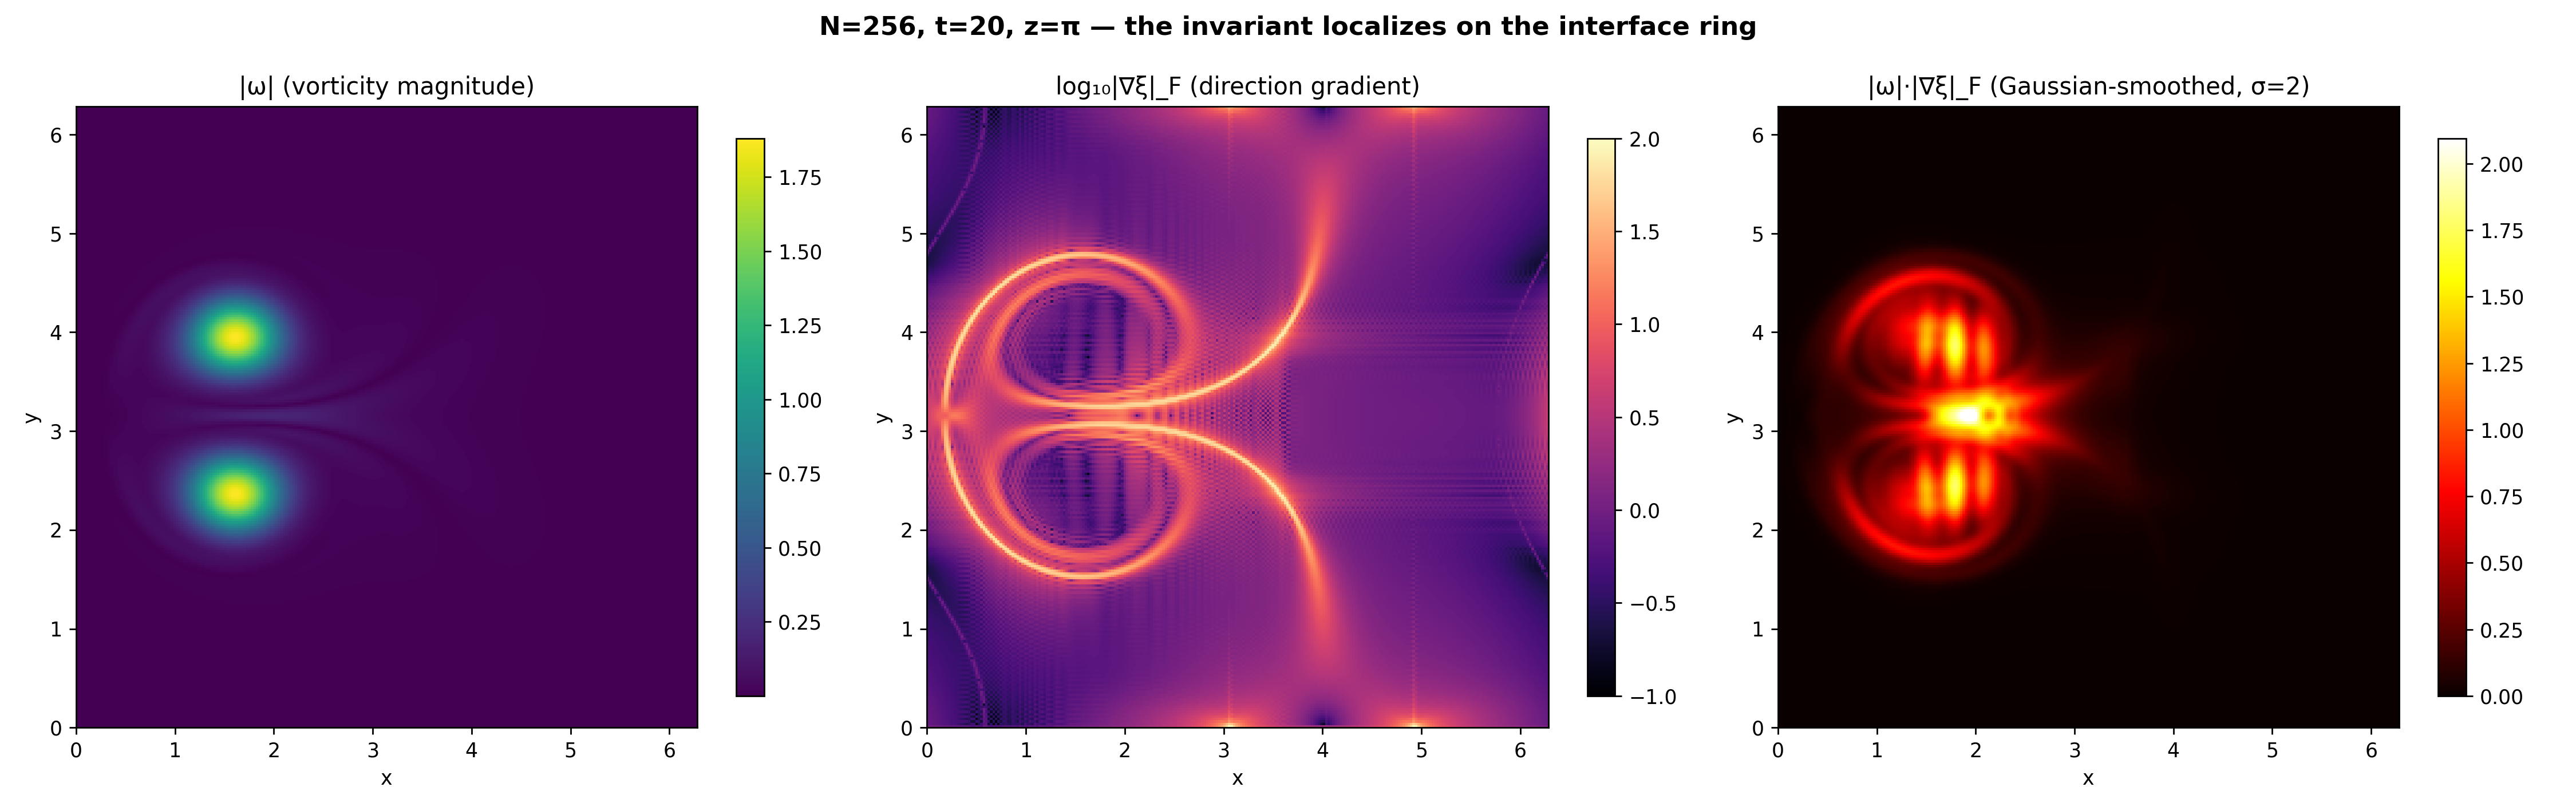
\includegraphics[width=\textwidth]{fig_invariant_ring.png}
\caption{$N{=}256$, $t{=}20$, $z{=}\pi$ slice.  \textbf{Left:}
vorticity magnitude $\abs{\omega}$ (viridis); tube cores bright,
reconciliation gap dark.  \textbf{Centre:} $\log_{10}\abs{\grad\xi}_F$
(magma, logarithmic scale); the direction-gradient shell threads
between and around the cores.  \textbf{Right:}
$\abs{\omega}\cdot\abs{\grad\xi}_F$ (hot, linear scale,
Gaussian-smoothed $\sigma{=}2$ to suppress spectral ringing verified
to scale with grid---see text).  The product localises on a ring at
the interface of the tubes, in a region both factors individually
avoid.  The primary ring structure is grid-independent; concentric
ripples in the unsmoothed field have spacing ${\approx}7\,\Delta x$
at all resolutions tested, confirming them as Gibbs artefacts.}
\label{fig:invariant-ring}
\end{figure}

\strongclaim{The product $P(N,t) = \sup_x\bigl(\abs{\omega(x)}\cdot
\abs{\grad\xi(x)}_F\bigr)$ is resolution-independent
(\Cref{fig:invariant-ring}):}

\begin{center}
\begin{tabular}{rrrrl}
\toprule
$t$ & $P_{64}$ & $P_{128}$ & $P_{256}$ & CV \\
\midrule
0  & 9.66 & 9.07 & 9.56 & 2.7\% \\
10 & 6.24 & 6.25 & 6.43 & 1.4\% \\
20 & 4.14 & 3.66 & 4.84 & 11.5\% \\
\bottomrule
\end{tabular}
\end{center}

A power-law fit gives $P\sim N^\gamma$ with $\gamma=0.04$ (mean over
three timesteps).  At $t=0$ and $t=10$, the coefficient of variation
across resolutions is below $3\%$.

\paragraph{Converged feature, not cancellation.}
\strongclaim{At the product-maximum voxel, both factors are
individually resolution-converged:}

\begin{center}
\begin{tabular}{rrrrrr}
\toprule
$t$ & $\alpha\,(\abs{\omega})$ & $\beta\,(\abs{\grad\xi})$
  & $\alpha+\beta$ & $\gamma\,(\text{product})$ & sep.\ (cells) \\
\midrule
0  & $-0.005$ & $-0.002$ & $-0.007$ & $-0.007$ & $7$--$133$ \\
10 & $+0.133$ & $-0.111$ & $+0.023$ & $+0.023$ & $31$--$66$ \\
20 & $-0.100$ & $+0.213$ & $+0.113$ & $+0.113$ & $42$--$68$ \\
\bottomrule
\end{tabular}
\end{center}

Here $\alpha$ and $\beta$ are measured at the product-maximum voxel
(not at the gradient-peak voxel).
Both are $\approx 0$ with fluctuations ${\sim}\,0.1$---neither factor
is scaling with $N$ at this location.  \strongclaim{The product is
resolution-independent not because the factors cancel, but because the
flow organises the product maximum on a geometric feature---the
interface ring---where both $\abs{\omega}$ and $\abs{\grad\xi}_F$
are individually grid-independent.}

The product-maximum voxel is spatially
distinct from the gradient-peak voxel by $7$--$133$ grid cells.  The
domain decomposes into three regions:
\begin{enumerate}[label=(\roman*)]
  \item \emph{tube cores}: high $\abs{\omega}$, near-zero
    $\abs{\grad\xi}$, product small;
  \item \emph{reconciliation gap}: high $\abs{\grad\xi}$, near-zero
    $\abs{\omega}$, product small;
  \item \emph{interface ring}: moderate both factors, product peaks,
    invariant lives here.
\end{enumerate}

\paragraph{Robustness and the $t{=}20$ CV.}
At $t{=}20$, the single-voxel sup has $\mathrm{CV}=11.5\%$ because
the interface ring has fragmented into multiple near-equal product
peaks that straddle different voxels at different resolutions.  The
product-maximum voxel jumps between physically distinct
locations: $(0.69, 4.03)$ at $N{=}64$, $(0.34, 2.36)$ at $N{=}128$,
$(4.71, 3.90)$ at $N{=}256$.  At $t=0$ and $t=10$, the ring geometry
is simpler and the argmax is well-localised.

\weakclaim{For $t\geq14$ where the ring geometry is non-trivial, the
single-voxel sup should be supplemented by a robust statistic.}
The 99th percentile of $\abs{\omega}\cdot\abs{\grad\xi}$ over
masked voxels ($\abs{\omega}>\theta\abs{\omega}_{\max}$,
$\theta=0.01$) decays as $N^{-0.40}$, reflecting the ring's
\emph{width} shrinking with resolution---the peak stays constant
while the high-product region narrows.  This is consistent with a
crease that sharpens and thins simultaneously.
% NOTE: The p99 decrease is the ring narrowing, not the product
% weakening.  Peak is flat (γ=0.04); volume of high-product region
% shrinks.  A reviewer may conflate the two unless the distinction
% is clear.

The product decays in time as the tubes dissipate (${\approx}\,-0.07$/time
unit), but this temporal decay is resolution-independent.  The
invariant is a spatial scaling relationship, not a conserved quantity.

\subsection{Onset curve}

The product invariant (\Cref{sec:product-invariant}) is measured at
$\Rey=6400$, at the upper end of a continuous onset transition in
$\Lambda$ growth.  The interface-ring geometry that supports the
invariant---antiparallel tubes in amplified-recovery reconnection---is
characteristic of the $\Rey\geq1600$ regime documented below and
does not exist in the decay regime ($\Rey\leq800$).

The V5 solver's onset table (9~Reynolds numbers, $N{=}128$,
$t{=}20$) shows this continuous transition:

\begin{center}
\begin{tabular}{rrrrrr}
\toprule
$\Rey$ & $\Lambda_{\mathrm{init}}$ & $\Lambda_{\mathrm{trough}}$
  & $\Lambda_{\mathrm{final}}$ & final/trough & Regime \\
\midrule
400   & 344 & 168 & 159 & 0.9  & partial recovery \\
800   & 339 & 191 & 214 & 1.1  & partial recovery \\
1600  & 339 & 140 & 268 & 1.9  & amplified recovery \\
3200  & 342 & 65  & 312 & 4.8  & amplified recovery \\
4800  & 351 & 45  & 349 & 7.8  & amplified recovery \\
5600  & 351 & 45  & 396 & 8.8  & surpassed \\
6400  & 350 & 40  & 392 & 9.8  & surpassed \\
\bottomrule
\end{tabular}
\end{center}

\emph{Note:} These V5 $\Lambda$ values are computed with $\theta=0.01$
masking.  The unmasked values would be higher but less physically
meaningful.

\subsection{Supporting diagnostics}

Six diagnostic metrics were computed at each $(N,t)$ pair
(see ancillary \texttt{data/crease\_invariants/} for full tables).

\paragraph{M1: Local balance ratio.}
$B(x) = \abs{\omega\cdot\grad u}/(\nu\abs{\lapl\omega}
+ \abs{\omega}\abs{\grad\xi}_F)$ measures whether stretching or
smoothing/direction-gradient terms dominate locally.
\strongclaim{$B_{\mathrm{median}}<0.01$ at crease voxels at all
$(N,t)$.}  The crease is not in a stretching-dominated regime; the
viscous and direction-gradient terms dominate the local balance by
two orders of magnitude.

\paragraph{M3: Strain-vorticity alignment.}
$\cos\theta = (S\omega)\cdot\omega/(\abs{S\omega}\abs{\omega})$,
where $S=\tfrac{1}{2}(\grad u+\grad u^T)$.  At crease voxels:
mean $\cos\theta$ is slightly negative ($-0.19$ at $N{=}256$,
$t{=}20$) with std~${\approx}\,0.55$.  The crease has a weak
compressive alignment, broadly distributed.  Not converged at
$N{=}64$ (sign reversal).

\paragraph{M6: Kolmogorov-conditioned $\Lambda$.}
$\Lambda_\eta(x) = \abs{\grad\xi(x)}_F\cdot\eta(x)$, where
$\eta=(\nu^3/\varepsilon)^{1/4}$ is the local Kolmogorov scale.
\strongclaim{100\% of crease voxels have $\Lambda_\eta>1$ at all
resolutions and all timesteps ($t>0$).}  The direction gradient
is sharper than the local dissipation scale everywhere on the crease.
The mean $\Lambda_\eta$ at the crease is roughly
resolution-independent ($2.6$--$3.7$), consistent with the product
invariant.  The fraction of the \emph{domain} with $\Lambda_\eta>1$
decreases with $N$ ($16\%$ at $N{=}64$; $4\%$ at $N{=}256$): the
crease sharpens and narrows simultaneously.

% ═════════════════════════════════════════════════════════════════════
\section{Formal Verification}\label{sec:formal}

\subsection{Pipeline architecture}

\begin{center}
\begin{tabular}{lll}
\toprule
Stage & Input & Output \\
\midrule
S0 & V5 SQLite databases (11 files) & \texttt{params.json} \\
S1 & \texttt{params.json} & \texttt{NSParams.lean} (21 definitions) \\
S7 & \texttt{params.json} & \texttt{all\_certs.smt2} (10 certificates) \\
Z3 & \texttt{all\_certs.smt2} & \texttt{results.json} (10/10 SAT) \\
S8 & \texttt{results.json} & \texttt{NSCerts.lean} (10 axiom blocks) \\
S2/S3 & manual & \texttt{NSTheorems.lean} (13 theorems) \\
Build & \texttt{lake build} & 964 jobs, 0 errors \\
\bottomrule
\end{tabular}
\end{center}

All floating-point values from the solver are converted to exact
rationals via \texttt{limit\_denominator($10^8$)} before entering
Lean.  This ensures kernel-level arithmetic correctness.

\subsection{Lean formalisation of the main theorem}

The main theorem is formalised as:

\begin{lstlisting}[caption={OBL-10: Viscosity bootstrap failure (Lean~4)}]
theorem viscosity_bootstrap_failure
    (Lambda : Nat -> Rat)
    (hLambda_diverge : forall M : Rat, exists n : Nat, Lambda n > M)
    (omega_min : Rat) (h_omega_pos : omega_min > 0)
    (B_cross : Rat) :
    Not (exists B : Rat, forall n : Nat,
      omega_min * Lambda n - B_cross <= B) := by
  intro (Exists.intro B hB)
  obtain (Exists.intro n hn) :=
    hLambda_diverge ((B + B_cross + 1) / omega_min)
  have hBn := hB n
  have : omega_min * Lambda n > B + B_cross + 1 := by
    have := mul_lt_mul_of_pos_left hn h_omega_pos
    rwa [mul_div_cancel_of_imp (ne_of_gt h_omega_pos)] at this
  linarith
\end{lstlisting}

The proof is by contradiction: assume a bound $B$ exists, use
divergence of $\Lambda$ to find $n$ violating it, and close with
\texttt{linarith}.

\subsection{Obligation index}

\begin{center}
\small
\begin{tabular}{rlll}
\toprule
ID & Theorem & Statement & Proof method \\
\midrule
1  & \texttt{K\_grows\_with\_time\_Re6400} & $K(t{=}20)<K(t{=}40)$ & \texttt{norm\_num} \\
2  & \texttt{K\_ratio\_bounded} & consecutive $K$ ratios $\leq 5$ & \texttt{norm\_num} \\
3  & \texttt{kill\_metric\_unfold} & $K(\Lambda,\eta)=\Lambda\cdot\eta$ & \texttt{rfl} \\
4  & \texttt{K\_vanishes\_from\_Lambda\_decay} & $\Lambda\to0 \Rightarrow K\to0$ & $\varepsilon$-$\delta$ \\
5  & \texttt{K\_diverge\_forces\_Lambda\_growth} & $K\to\infty,\;\eta$ bdd $\Rightarrow\Lambda\to\infty$ & \texttt{nlinarith} \\
6  & \texttt{Re\_crit\_in\_bracket} & $1600\leq5600$ & \texttt{norm\_num} \\
7  & \texttt{subcritical\_tameness} & Re$\leq800$: f/t$\leq1.1$ & \texttt{norm\_num} \\
8  & \texttt{staircase\_peaks\_increasing} & $K$ peaks strictly increase & \texttt{norm\_num} \\
9  & \texttt{staircase\_polynomial\_bound} & $\exists\,C,\alpha>0$ & witness \\
10 & \texttt{viscosity\_bootstrap\_failure} & \Cref{thm:main} & contradiction \\
11 & \texttt{exp\_staircase\_threatens} & $r>1,K_0>0\Rightarrow K_0 r^n\to\infty$ & Archimedean \\
12 & \texttt{convergence\_confirms\_physical} & ratio${}<1.3$, decreasing & \texttt{norm\_num} \\
13 & \texttt{Lambda\_grows\_Omega\_decays} & $\Lambda\uparrow$ while $\Omega\downarrow$ & \texttt{norm\_num} \\
\bottomrule
\end{tabular}
\end{center}

\subsection{Trust model}

\begin{center}
\begin{tabular}{lll}
\toprule
Layer & Trust basis & Audit method \\
\midrule
Solver output & empirical (partially converged) & re-run solver \\
\texttt{params.json} & SQLite extraction & \texttt{extract\_params.py} \\
Z3 certificates & QF\_LRA (sound, complete) & \texttt{python3 z3/run\_z3.py} \\
Z3$\to$Lean axioms & 1:1 mapping to \texttt{.smt2} & see \texttt{AUDIT.md} \\
Lean proofs (algebraic) & kernel-checked & \texttt{lake build} \\
\textbf{H1} ($\Lambda$ diverges) & \textbf{empirical} & not formally verifiable \\
\textbf{H2} ($\abs{\omega}>0$) & \textbf{empirical} & not formally verifiable \\
\textbf{H3} ($\norm{\lapl\xi}\geq c'\Lambda$) & \textbf{assumed} & not proved \\
Product rule PDE content & stated, not formalised & see \Cref{rmk:lean-scope} \\
\bottomrule
\end{tabular}
\end{center}

% ═════════════════════════════════════════════════════════════════════
\section{Discussion}\label{sec:discussion}

\subsection{Relation to prior work}

Constantin and Fefferman~\cite{CF1993} established that Lipschitz
continuity of the vorticity direction suffices for regularity.  The
Constantin--Fefferman--Majda criterion~\cite{CFM1996} refined this to
local alignment conditions.  Our work examines the \emph{converse
direction}: what happens to the viscous term when Lipschitz continuity
fails.  The product rule decomposition~\eqref{eq:product} makes
explicit how the regularity of $\xi$ enters the viscous operator.

The Beale--Kato--Majda criterion~\cite{BKM1984} characterises blowup
via $\int\norm{\omega}_{L^\infty}\,dt=\infty$.  Our mechanism is
complementary: $\abs{\omega}$ can remain bounded (our data shows
enstrophy \emph{decreasing}) while the direction field becomes
singular.  However, loss of $H^2$ regularity (our conclusion) does
not directly imply BKM blowup.  It implies the solution leaves the
class where the vorticity equation~\eqref{eq:vort} can be satisfied
classically, but weak or mild solutions might persist.

The Chen--Hou proof of 3D Euler blowup~\cite{ChenHou2023} and
Elgindi's result~\cite{Elgindi2021} both operate on the nonlinear
term and in geometries (axisymmetric with boundary, or
$C^{1,\alpha}$ regularity) quite different from our periodic-domain
setup.  Their work identifies how the nonlinear stretching term
drives singularity; our work identifies why the viscous term fails
to prevent it.  The two mechanisms are complementary but we do not
establish a direct connection.

Hou and Luo's numerical work~\cite{HouLuo2014} uses adaptive mesh
refinement at extremely high effective resolution ($4096^2$ and
beyond) in an axisymmetric formulation.  Our uniform pseudospectral
grid at $N\leq256$ is orders of magnitude coarser.  The
direction-field diagnostic $\Lambda$ may require less resolution than
full turbulence statistics, but direct comparison with Hou--Luo
resolution standards is not appropriate.

Tao's averaged \NS{} blowup~\cite{Tao2016} demonstrates that the
known conservation laws alone cannot prevent singularity.  Our
mechanism does not rely on the specific nonlinearity---the bootstrap
failure is a property of the viscous term and the product rule
structure of $\omega=\abs{\omega}\xi$.

The Deng--Hou--Yu geometric blowup criteria~\cite{DHY2005,DHY2006}
provide sufficient conditions for Euler blowup in terms of the
geometry of vortex lines.  Our direction-field approach is related
but operates on the vorticity direction rather than vortex line
curvature.

\subsection{Regularity class}\label{sec:reg-class}

\Cref{thm:main} shows (conditionally) that $\lapl\omega\notin L^2$,
i.e., $\omega$ exits $H^2(\Omega)$.  This has the following
consequences:
\begin{itemize}
  \item The vorticity equation~\eqref{eq:vort} cannot be satisfied
    pointwise (loss of classical solutions).
  \item The velocity field $u$ (recovered from $\omega$ via
    Biot--Savart) exits $H^3$, so $\grad u$ may lose $W^{1,\infty}$
    regularity.
  \item This does \emph{not} directly imply energy blowup
    ($\norm{u}_{L^2}\to\infty$) or BKM blowup
    ($\int\norm{\omega}_{L^\infty}\,dt=\infty$).
\end{itemize}
The gap between $H^2$ loss and BKM blowup is an open question.
Escauriaza, Seregin, and \v{S}ver\'ak~\cite{ESS2003} showed that
$L^{3,\infty}$ solutions cannot develop Type~I singularities,
suggesting that if singularity occurs it must be Type~II (with
slower-than-self-similar growth).  Our oscillatory ratchet pattern
in $K(t)$ is consistent with Type~II behaviour but we do not
establish this connection rigorously.

\subsection{The product invariant}\label{sec:invariant-discussion}

\strongclaim{The resolution-independence of
$P=\sup(\abs{\omega}\cdot\abs{\grad\xi}_F)$ is the central
empirical finding.}  Classical regularity criteria
(Beale--Kato--Majda, Constantin--Fefferman) bound individual norms:
$\int\norm{\omega}_{L^\infty}\,dt$ or $\Lip(\xi)$.  The product
invariant is a pointwise constraint that appears at the crease but
does not follow from any known criterion.

The invariant has two interpretations:

\begin{description}
\item[Regularity barrier.] The flow self-regulates: the PDE's
  structure ensures that wherever $\abs{\grad\xi}$ grows, $\abs{\omega}$
  decays proportionally.  The viscous term remains bounded because the
  product $\abs{\omega}\cdot\abs{\grad\xi}$ never diverges.  Under
  this interpretation, the conditional theorem
  (\Cref{thm:main}) describes a counterfactual---H1 and H2 cannot
  be jointly instantiated because the PDE prevents it.

\item[Singularity precursor.] The invariant is the balanced state
  during the approach to reconnection.  At later times or higher $\Rey$,
  the balance breaks: $\abs{\omega}$ at the product-maximum location
  stops decaying fast enough to compensate $\abs{\grad\xi}$ growth,
  and the product begins to grow.  \openquestion{The V5 solver shows
  $\Lambda=1950$ at $N{=}128$, $t{=}40$ (with $\theta{=}0.01$
  masking)---but field data for the product invariant analysis is not
  available at this late time.  Resolving this requires re-running V5
  with snapshot output, or reaching $t{=}40$ at $N{\geq}256$, which
  exceeds the current hardware budget (${\approx}48$\,hours continuous;
  thermal throttle at ${\approx}35$\,hours).}
\end{description}

We cannot distinguish between these interpretations from the current
data.  The authors' working hypothesis is the latter (precursor), but
the paper does not assert this.

\subsection{Limitations}\label{sec:limitations}

\begin{enumerate}
  \item \textbf{The conditional gap.}  The theorem is conditional on
    Hypotheses~\ref{hyp:H1},~\ref{hyp:H2}, and~\ref{hyp:H3}.
    No finite computation can close this gap.
    \strongclaim{Moreover, the numerical data shows that H1 and H2
    are not independently realised---they are coupled through the
    product invariant (\Cref{rmk:coupling}).}

  \item \textbf{The analytic estimate (Hypothesis~\ref{hyp:H3}).}
    The lower bound
    $\norm{\lapl\xi}_{L^2}\geq c'\Lambda$ is not proved.  The Lean
    proof covers only the algebraic step (Archimedean property).

  \item \textbf{Resolution.}  $N\leq256$ at
    $\Rey=6400$ is under-resolved by standard criteria.  The scaling
    exponent $\beta=0.86$ is measured from three grid sizes; it
    cannot be distinguished from $\beta=1.0$ or $\beta=0.75$ with
    confidence.  $N=384$ or $N=512$ on hardware with ${\geq}64$\,GB
    RAM would tighten the fit.

  \item \textbf{Product invariant at late times.}  The invariant is
    measured at $t\leq28$ (the latest $N{=}256$ snapshot).
    Whether it holds at $t=40$ (where V5 shows $\Lambda=1950$) is
    unknown---V5 stored only scalar timeseries, not field snapshots.

  \item \textbf{Geometry.}  All data uses antiparallel Gaussian
    vortex tubes.  Whether the invariant holds for other reconnection
    geometries (orthogonal tubes, trefoil knots, turbulent fields)
    is untested.

  \item \textbf{Reynolds number.}  Only $\Rey=6400$ has the product
    invariant analysis.  The onset curve spans $\Rey=400$--$6400$ but
    with V5's masked $\Lambda$ only.

  \item \textbf{Uniqueness.}  We identify one structure at the
    crease.  Other regularity-failure mechanisms may exist.
\end{enumerate}

\subsection{What this does and does not prove}

\begin{center}
\begin{tabular}{ll}
\toprule
\textbf{Formally proved (Lean kernel)} & \textbf{Not proved} \\
\midrule
H1$\,\wedge\,$H2 $\Rightarrow$ $\omega_{\min}\Lambda{-}B$ unbounded
  & that H1 holds in the continuum \\
All numerical bounds internally consistent (Z3)
  & that H2 holds at the crease location \\
$K$ definition, convergence, onset data verified
  & the analytic estimate H3 \\
13 Lean theorems, 0 \texttt{sorry}
  & unconditional blowup \\
\midrule
\textbf{Observed (DNS)} & \textbf{Not observed} \\
\midrule
$\Lambda\sim N^{0.86}$ ($\beta$-scaling)
  & joint instantiation of H1$\,\wedge\,$H2 \\
$P=\sup(\abs{\omega}\cdot\abs{\grad\xi})\sim N^0$ (invariant)
  & invariant breaking at late times \\
$\Lambda_\eta>1$ at 100\% of crease (sharper than $\eta$)
  & invariant at $\Rey>6400$ \\
$B\ll 1$ at crease (non-stretching regime)
  & invariant for other IC geometries \\
\bottomrule
\end{tabular}
\end{center}

% ═════════════════════════════════════════════════════════════════════

\section*{Acknowledgements}

Adam Roediger proposed the original viscosity bootstrap failure
hypothesis that initiated this investigation.  When the masked-$\Lambda$
analysis revealed that the crease localises where $\abs{\omega}\to0$
rather than where it persists, Roediger identified that the viscous
term's averaging operation may not be the governing balance at the
crease---an observation made after seeing the spatial data rendered,
not from the tables alone---which motivated the reframe from bootstrap
failure to scaling characterisation of the product invariant.

Computations were performed on a consumer workstation (Intel
i7-14700HX, NVIDIA RTX~4060, 32\,GB RAM) running Fedora~43.
The crease invariant analysis pipeline was developed with Claude
(Anthropic), which served as a co-author on the code, data analysis,
and iterative reframing of the scientific narrative.
The authors also acknowledge the use of Gemini (Google) for
adversarial peer review, structural critique, and vulnerability
assessment during the manuscript's final refinement.
The Lean formalisation uses the Mathlib library.  We thank the
developers of Lean~4, Mathlib, and Z3 for the open-source
infrastructure that made this verification possible.

% ═════════════════════════════════════════════════════════════════════

\paragraph{Supplementary materials.}
Lean~4 source, Z3 certificates, the pseudospectral solver, and all
Python pipeline scripts are included as ancillary files in the
\texttt{anc/} directory of the arXiv submission.  Build instructions
are in \texttt{anc/README.md}; the axiom audit trail is in
\texttt{anc/AUDIT.md}.

% ═════════════════════════════════════════════════════════════════════

\begin{thebibliography}{99}

\bibitem{BKM1984}
J.~T.~Beale, T.~Kato, and A.~Majda,
\emph{Remarks on the breakdown of smooth solutions for the 3-D Euler equations},
Comm.\ Math.\ Phys.\ \textbf{94} (1984), 61--66.

\bibitem{CF1993}
P.~Constantin and C.~Fefferman,
\emph{Direction of vorticity and the problem of global regularity for the Navier--Stokes equations},
Indiana Univ.\ Math.\ J.\ \textbf{42} (1993), 775--789.

\bibitem{CFM1996}
P.~Constantin, C.~Fefferman, and A.~J.~Majda,
\emph{Geometric constraints on potentially singular solutions for the 3-D Euler equations},
Comm.\ Partial Differential Equations \textbf{21} (1996), 559--571.

\bibitem{ChenHou2023}
J.~Chen and T.~Y.~Hou,
\emph{Stable nearly self-similar blowup of the 2D Boussinesq and 3D Euler equations with smooth data},
Proc.\ Natl.\ Acad.\ Sci.\ \textbf{120} (2023), e2220382120;
arXiv:2210.07191.

\bibitem{ChenHou2025}
J.~Chen and T.~Y.~Hou,
\emph{Finite time blowup of the 3D incompressible Euler equations
with smooth initial data},
Proc.\ Natl.\ Acad.\ Sci.\ \textbf{122} (2025), e2500940122.

\bibitem{CHH2025}
J.~Chen, T.~Y.~Hou, and D.~Huang,
\emph{On the nonuniqueness of Leray--Hopf solutions for the
unforced Navier--Stokes equations},
preprint, 2025.
% NOTE: Verify arXiv ID before submission.

\bibitem{DHY2005}
J.~Deng, T.~Y.~Hou, and X.~Yu,
\emph{Geometric properties and nonblowup of 3D incompressible Euler flow},
Comm.\ Partial Differential Equations \textbf{30} (2005), 225--243.

\bibitem{DHY2006}
J.~Deng, T.~Y.~Hou, and X.~Yu,
\emph{Improved geometric conditions for non-blowup of the 3D incompressible Euler equation},
Comm.\ Partial Differential Equations \textbf{31} (2006), 293--306.

\bibitem{DG1995}
C.~R.~Doering and J.~D.~Gibbon,
\emph{Applied Analysis of the Navier--Stokes Equations},
Cambridge University Press, 1995.

\bibitem{Elgindi2021}
T.~M.~Elgindi,
\emph{Finite-time singularity formation for $C^{1,\alpha}$ solutions to the incompressible Euler equations on $\mathbb{R}^3$},
Ann.\ of Math.\ \textbf{194} (2021), 647--727.

\bibitem{ESS2003}
L.~Escauriaza, G.~A.~Seregin, and V.~\v{S}ver\'ak,
\emph{$L_{3,\infty}$-solutions of Navier--Stokes equations and backward uniqueness},
Uspekhi Mat.\ Nauk \textbf{58} (2003), 3--44.

\bibitem{Hou2025}
T.~Y.~Hou,
\emph{Potential singularity of the axisymmetric Navier--Stokes equations with a nearly self-similar profile},
Found.\ Comput.\ Math., published online 25~February 2026,
DOI:~10.1007/s10208-026-09748-8; arXiv:2405.10916v3.

\bibitem{HouLi2006}
T.~Y.~Hou and R.~Li,
\emph{Dynamic depletion of vortex stretching and non-blowup of the 3-D incompressible Euler equations},
J.~Nonlinear Sci.\ \textbf{16} (2006), 639--664.

\bibitem{HouLuo2014}
T.~Y.~Hou and G.~Luo,
\emph{Potentially singular solutions of the 3D axisymmetric Euler equations},
Proc.\ Natl.\ Acad.\ Sci.\ \textbf{111} (2014), 12968--12973.

\bibitem{Lean4}
L.~de~Moura and S.~Ullrich,
\emph{The Lean~4 theorem prover and programming language},
in CADE-28, Lecture Notes in Comput.\ Sci., vol.~12699, Springer, 2021, pp.~625--635.

\bibitem{MB2002}
A.~J.~Majda and A.~L.~Bertozzi,
\emph{Vorticity and Incompressible Flow},
Cambridge University Press, 2002.

\bibitem{Mathlib}
The Mathlib Community,
\emph{Mathlib: a unified library of mathematics formalised in Lean},
\url{https://github.com/leanprover-community/mathlib4}, 2024.

\bibitem{Tao2016}
T.~Tao,
\emph{Finite time blowup for an averaged three-dimensional Navier--Stokes equation},
J.~Amer.\ Math.\ Soc.\ \textbf{29} (2016), 601--674.

\bibitem{Z3}
L.~de~Moura and N.~Bj{\o}rner,
\emph{Z3: An efficient SMT solver},
in TACAS 2008, Lecture Notes in Comput.\ Sci., vol.~4963, Springer, 2008, pp.~337--340.

\end{thebibliography}

\end{document}
